%% =============================================================================
%% The CGAL User Manual
%% Chapter: Geometric Optimization
%% -----------------------------------------------------------------------------
%% file   : doc_tex/basic/Optimization/user_part.tex
%% package: Optimisation_doc
%% author : Sven Sch�nherr <sven@inf.ethz.ch>
%% -----------------------------------------------------------------------------
%% $Id$
%% $Date$
%% =============================================================================

%%\section{Introduction}

Geometric optimization deals with problems of computing geometric
objects which are optimal subject to certain criteria and constraints.
Our running example will be the problem of computing the sphere of
smallest radius which contains a given point set in $d$-dimensional
Euclidean space.

\begin{ccHtmlOnly}
<center>
<img border="0" src="ball.gif" align="center">
</center>
\end{ccHtmlOnly} 

\begin{ccTexOnly}
\begin{center}
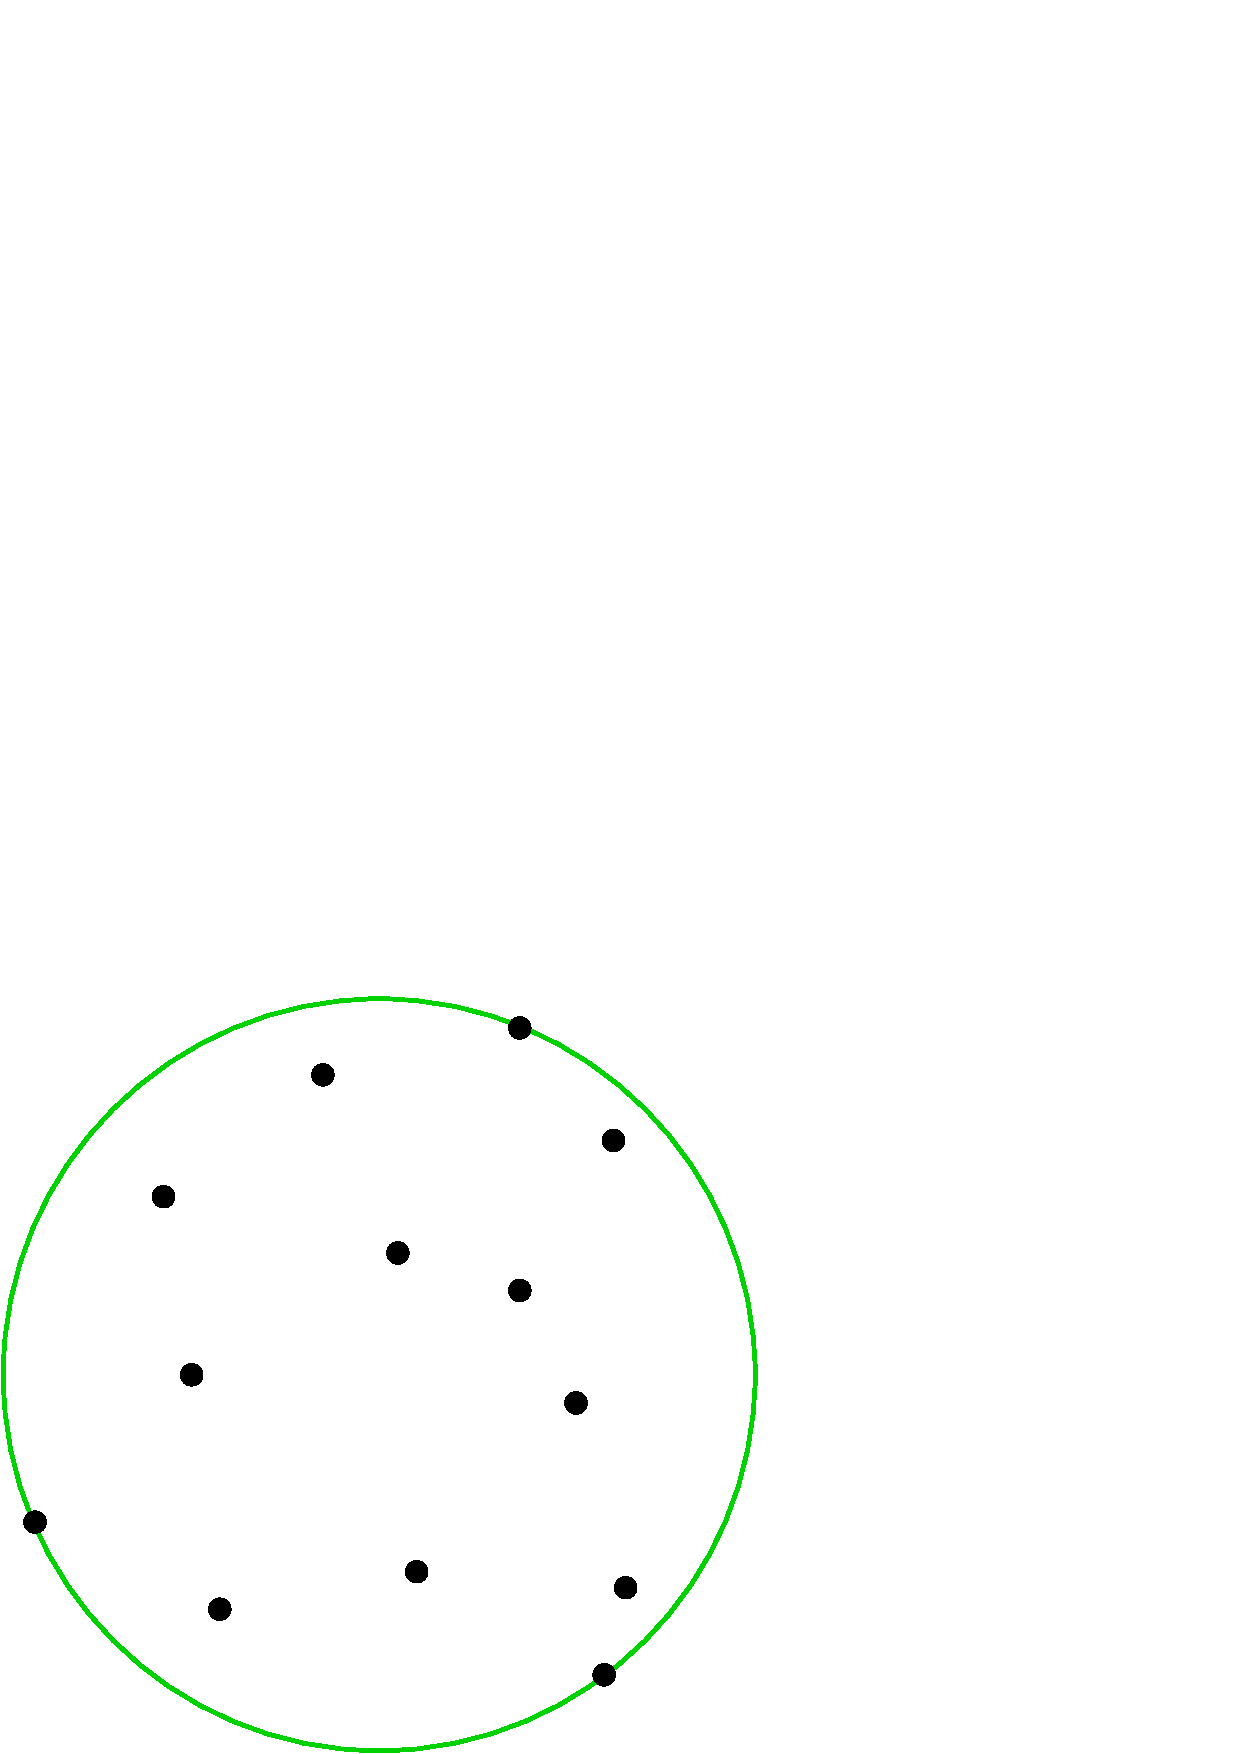
\includegraphics[width=4cm]{Optimisation/ball}
%%\leavevmode\epsfxsize8cm\epsffile{ball.eps}
\end{center}
\end{ccTexOnly}

The geometric optimization algorithms in \cgal\ fall into three categories,
``Bounding Volumes'', ``Optimal Distances'' and ``Advanced Techniques''.

\section{Bounding and Inscribed Volumes\label{c:opt:sec:bounding}}

This category contains algorithms which for a given point set compute
the ``best'' circumscribing (or inscribed) object from a specific
class. If the class consists of all spheres in $d$-dimensional
Euclidean space and ``best'' is defined as having smallest radius,
then we obtain the smallest enclosing sphere problem already mentioned
above.

In the following example a smallest enclosing circle
(\ccc{CGAL::Min_circle_2<Traits>}) is constructed from points 
on a line and written to standard output. The example
shows that it is advisable to switch on random shuffling 
in order to deal with a `bad' order of the input points. 
%%The default traits class is used here.

\ccIncludeVerbatim{Min_circle_2/Min_circle_2_simple_demo.cpp}

Other classes for which we provide solutions are ellipses
(\ccc{CGAL::Min_ellipse_2<Traits>}), rectangles
(\ccc{CGAL::min_rectangle_2}), parallelograms
(\ccc{CGAL::min_parallelogram_2}) and strips (\ccc{CGAL::min_strip_2})
in the plane, with appropriate optimality criteria. For arbitrary
dimensions we provide smallest enclosing spheres for points
(\ccc{CGAL::Min_sphere_d<Traits>}) and spheres for spheres
(\ccc{CGAL::Min_sphere_of_spheres_d<Traits>}), smallest enclosing
annuli (\ccc{CGAL::Min_annulus_d<Traits>}), and approximate
minimum-volume enclosing ellipsoid with user-specified
approximation ratio (\ccc{CGAL::Approximate_min_ellipsoid_d<Traits>}).

\begin{ccHtmlOnly}
<center>
<img border="0" src="annulus.gif" align="center">
</center>
\end{ccHtmlOnly} 

\begin{ccTexOnly}
\begin{center}
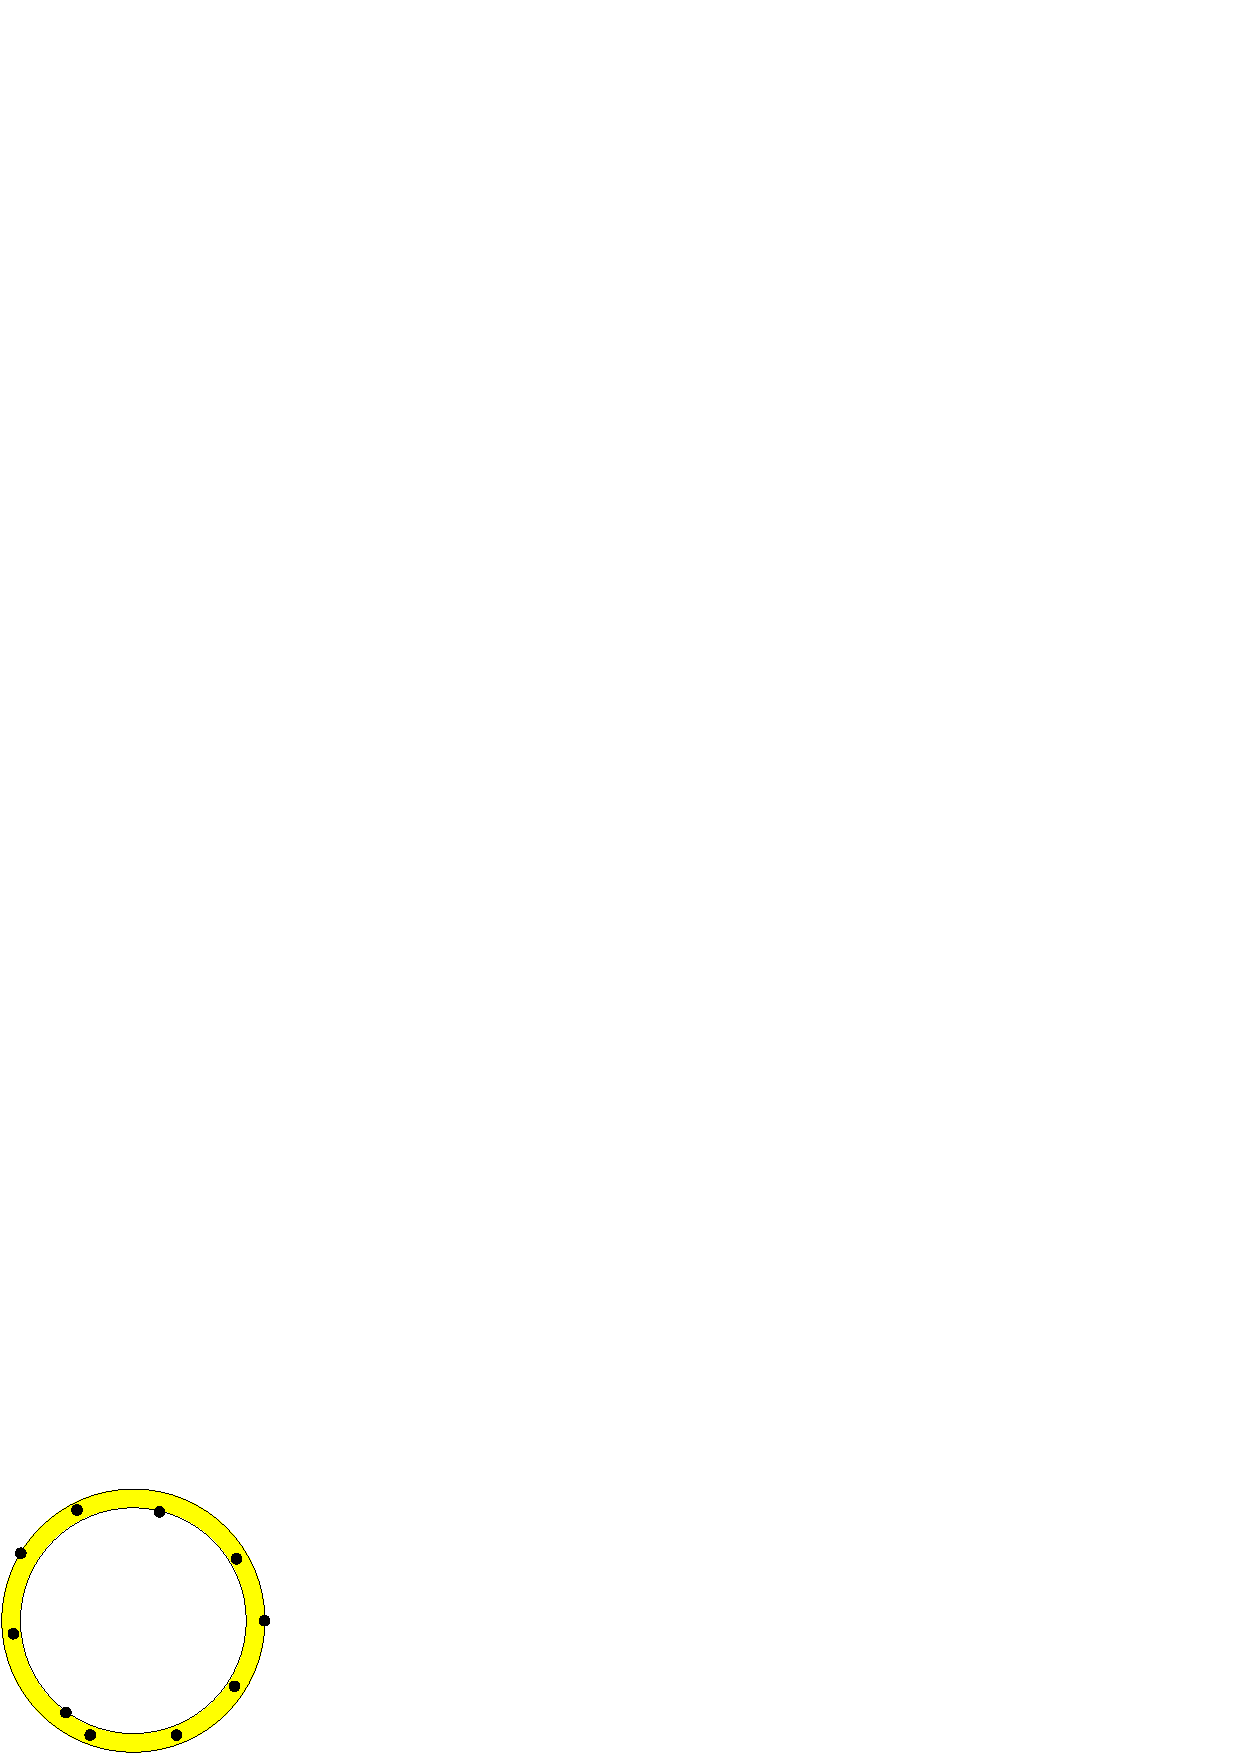
\includegraphics[width=4cm]{Optimisation/annulus}
%%\leavevmode\epsfxsize8cm\epsffile{annulus.eps}
\end{center}
\end{ccTexOnly}

Bounding volumes can be used to obtain simple approximations of
complicated objects. For example, consider the problem of deciding
whether two moving polygons currently intersect. An obvious solution
is to discretize time and perform a full intersection test for any
time step. If the polygons are far apart most of the time, this is
unnecessary. Instead, simple bounding volumes (for examples, circles)
are computed for both polygons at their initial positions. At
subsequent time steps, an intersection test between the moving
bounding circles replaces the actual intersection test; only if the
circles do intersect, the expensive intersection test between the
polygons is performed. In practice, bounding volume hierarchies are
often used on top of simple bounding volumes to approximate
complicated objects more accurately.

As far as inscribed volumes are concerned, we provide algorithms for
computing maximal inscribed $k$-gons (triangles, quadrilaterals,
\dots) of a planar point set $P$. Maximal $k$-gons are convex, and it
is known that their vertices can be chosen to be vertices of the
convex hull of $P$. Hence, the functions
\ccc{CGAL::maximum_area_inscribed_k_gon_2} and
\ccc{CGAL::maximum_perimeter_inscribed_k_gon_2} operate on convex polygons
only. The example below shows that the largest area triangle (green)
and the largest perimeter triangle (orange, containing the top point)
of a point set are different in general.

\begin{ccHtmlOnly}
<center>
<img border="0" src="max_triangle.gif" align="center">
</center>
\end{ccHtmlOnly} 

\begin{ccTexOnly}
\begin{center}
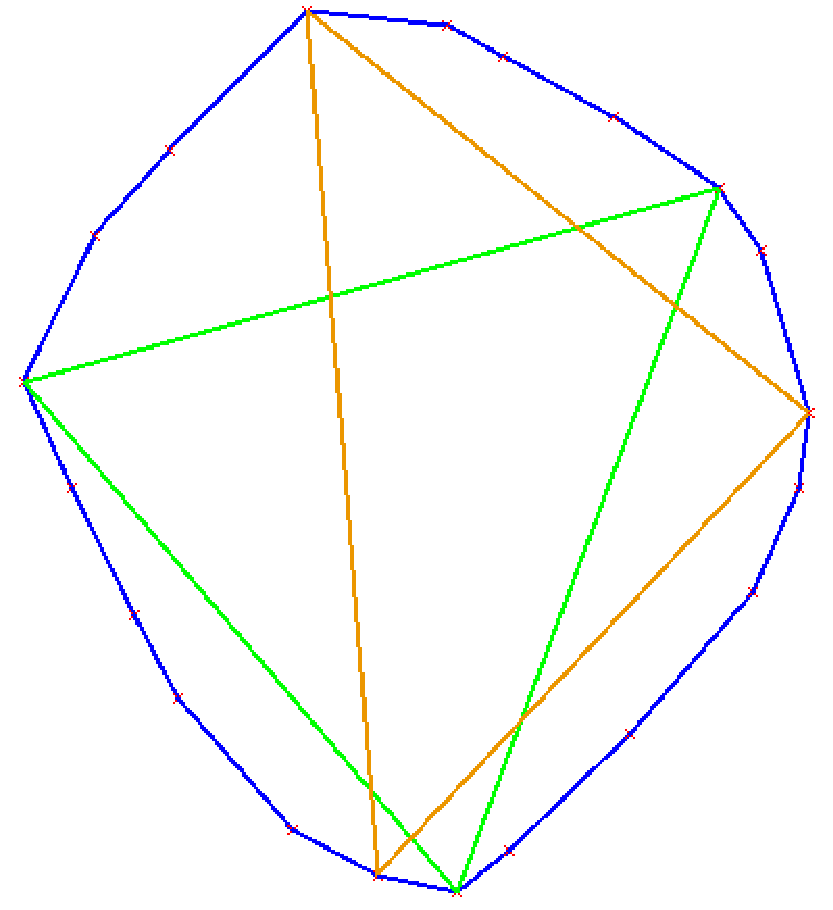
\includegraphics[width=5cm]{Optimisation/max_triangle}
\end{center}
\end{ccTexOnly}


We further provide an algorithm for computing the maximal area
inscribed axis parallel rectangle 

Given a set of points in the plane, the class \ccc{CGAL::Largest_empty_iso_rectangle_2<T>}
is a data structure that maintains an iso-rectangle with the largest area among
all iso-rectangles that are inside a given iso-rectangles, and
that do not contain any point of the point set.

\begin{ccHtmlOnly}
<center>
<img border="0" src="largestEmptyRect.gif" align="center">
</center>
\end{ccHtmlOnly} 

\begin{ccTexOnly}
\begin{center}
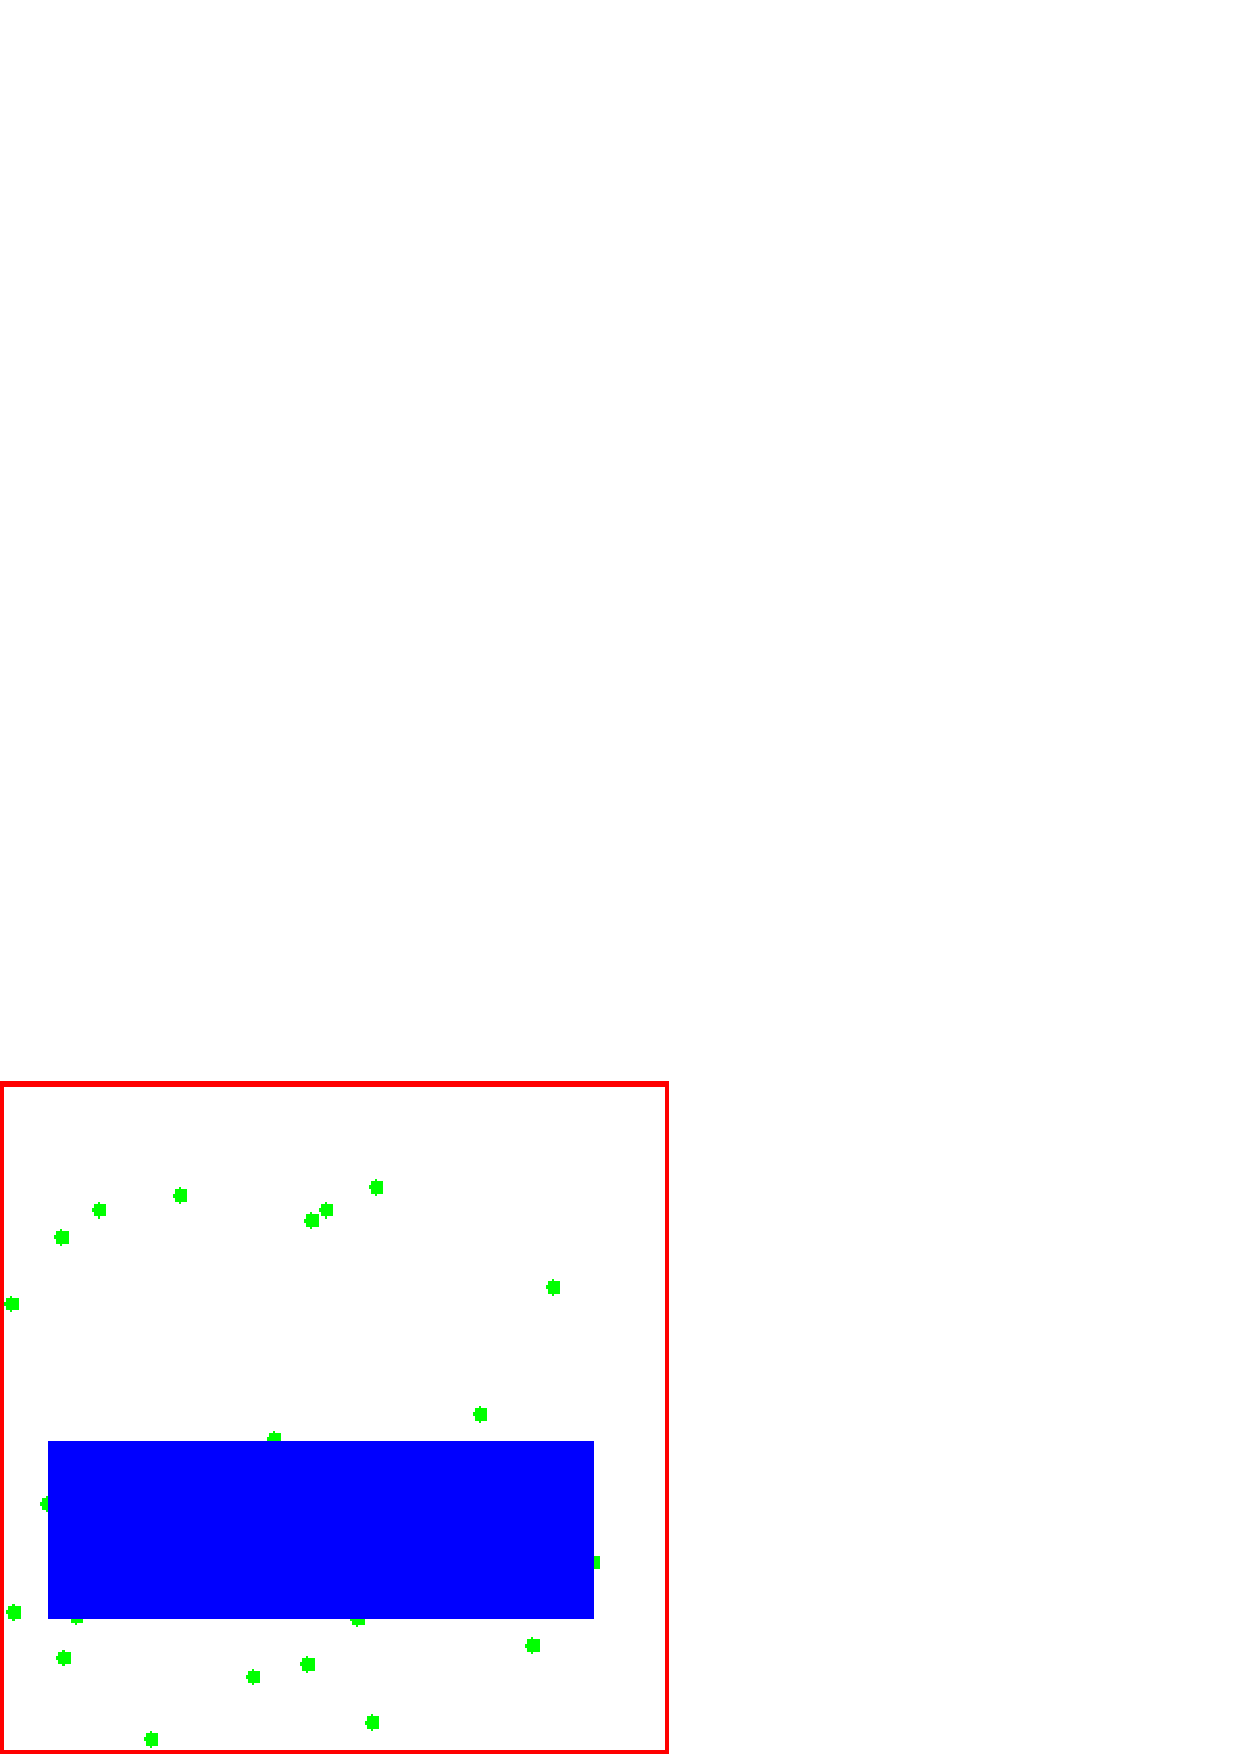
\includegraphics[width=5cm]{Optimisation/largestEmptyRect}
\end{center}
\end{ccTexOnly}

Bounding and inscribed volumes are also frequently applied to extract
geometric properties of objects. For example, the smallest enclosing
annulus of a point set can be used to test whether a set of points is
approximately cospherical. Here, the width of the annulus (or its
area, or still another criterion that we use) is a good measure for
this property. The largest area triangle is for example used in
heuristics for matching archaeological aerial photographs. Largest
perimeter triangles are used in scoring cross country soaring flights,
where the goal is basically to fly as far as possible, but still
return to the departure airfield. To score simply based on the total
distance flown is not a good measure, since circling in thermals
allows to increase it easily.

Bounding volumes also define geometric ``center points'' of objects.
For example, if two objects are to be matched (approximately), one
approch is to first apply the translation that maps the centers of
their smallest enclosing spheres onto each other.  Simpler centers are
possible, of course (center of gravity, center of bounding box), but
more advanced bounding volumes might give better results in some
cases. It can also make sense to consider several center points
instead of just one. For example, we provide algorithms to cover a
planar point set with between two and four minimal boxes
(\ccc{CGAL::rectangular_p_center_2}). Below is an example covering with
three boxes; the center points are shown in red.

\begin{ccHtmlOnly}
<center>
<img border="0" src="pcenter.gif" align="center">
</center>
\end{ccHtmlOnly} 

\begin{ccTexOnly}
\begin{center}
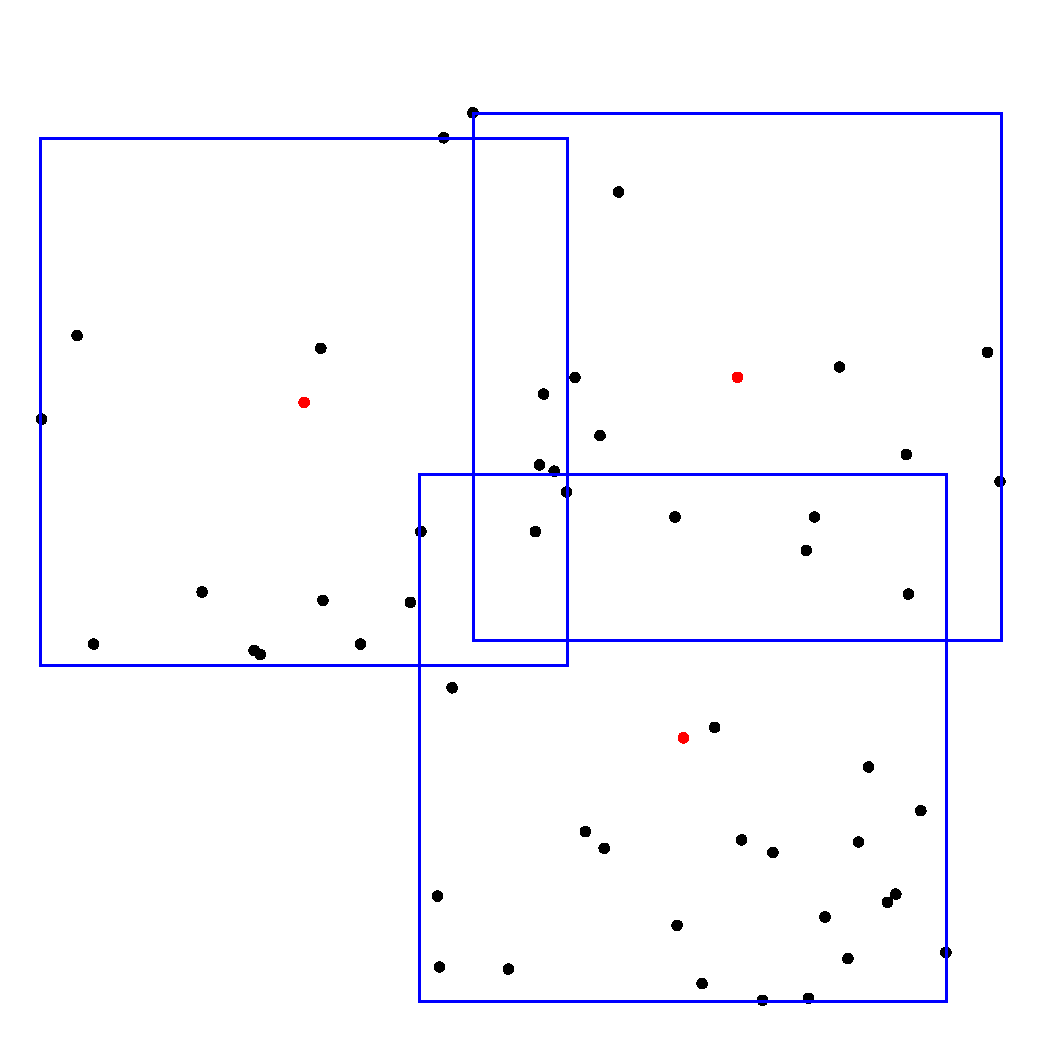
\includegraphics[width=5cm]{Optimisation/pcenter}

\end{center}
\end{ccTexOnly}

%To avoid later disappointment: one very nice class of bounding
%volumes, namely ellipsoids in three- and higherdimensional space, is
%currently not supported by \cgal. The reason is that the algebraic
%complexity of this problem is still beyond the level which would allow
%us to come up with a solution that satisfies the \cgal\ standards. We
%are working on a solution for 3-space, though.

\section{Optimal Distances}

This section currently consists of two algorithms only. On one hand,
one can compute the computation of the distance between the convex
hulls of two given point sets in $d$-dimensional Euclidean space
(\ccc{CGAL::Polytope_distance_d<Traits>}). Moreover, it is possible to
compute the width of a point set in three dimensions
(\ccc{CGAL::Width_3<Traits>}).

\begin{ccHtmlOnly}
<center>
<img border="0" src="polydist.gif" align="center">
</center>
\end{ccHtmlOnly} 

\begin{ccTexOnly}
\begin{center}
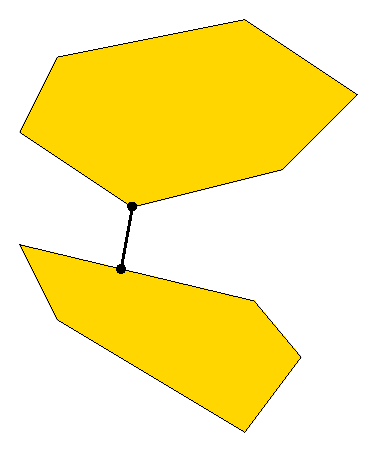
\includegraphics[width=4cm]{Optimisation/polydist}
\end{center}
\end{ccTexOnly}

The obvious application is collision detection between convex bodies
in space. In the spirit of the bounding volume application above, it
also makes sense for nonconvex objects: a full intersection test
between complicated objects could in a first stage be approximated
with the test between the convex hulls of the objects. Only if the
hulls intersect, a full intersection test is necessary.

To dampen fears concerning the performance of the distance
computation, we want to mention that the convex hulls of the input
point sets are not explicitly computed. This avoids a runtime which
grows exponentially in $d$. In fact, the runtime is almost always
linear in the size of the two point sets.

\section{Monotone and Sorted Matrix Search}

%% Geometric optimization is a well-studied subject also in theory.
%% Consequently, general design principles have been developed from which
%% solutions to diverse problems arise. For example, although the
%% problems of computing the smallest enclosing sphere of a point set and
%% the problem of computing the distance between two convex hulls seem to
%% be quite different, they are both instances of a more general
%% optimization problem, named ``quadratic programming''. To be more
%% specific, \cgal's solutions for the two quadratic programming
%% instances just mentioned are based on a general quadratic programming
%% solver, which will be documented as a separate unit in future
%% releases.

%% This section provides interfaces to several such general techniques as
%% well as additional concrete optimization algorithms that derive from
%% these general techniques.

%% To be more specific, \cgal's solutions for the two quadratic
%% programming instances just mentioned are based on a general quadratic
%% programming solver, which itself is available as an advanced
%% technique.  This means, using \cgal, you can solve your favorite
%% quadratic program, even if it does not assume the form of one of the
%% optimization problems that we explicitly address! A word of warning is
%% in order: the interface of the quadratic programming solver has mainly
%% been developed for internal use by the \cgal\ developers community. In
%% particular, feedback from the developers has influenced (and will
%% further influence) its design. This means: you are welcome to use the
%% solver's interface, but if you do so, please be aware that it might
%% change in the future, making adaptions of your code necessary. In the
%% future, the interface and the functionality will stabilize.


\ccc{CGAL::monotone_matrix_search} and \ccc{CGAL::sorted_matrix_search} 
are techniques that deal with the problem of efficiently finding
largest entries in matrices with certain structural properties. Many
concrete problems can be modelled as matrix search problems, and for
some of them we provide explicit solutions that allow you to solve
them without knowing about the matrix search technique. Examples are,
the computation of all furthest neighbors for the vertices of a convex
polygon, maximal $k$-gons inscribed into a planar point set, and
computing rectangular $p$-centers.

%% ===== EOF ===================================================================



